% Chapter 2

\chapter{Estado da Arte}	%The main chapter title
\chaptermark{Estado da Arte}	%Short version for page header. Comment if not needed
\label{Chapter2}	%For referencing the chapter elsewhere, use \ref{Chapter2} 

Neste capitulo é apresentado várias arquiteturas de \textit{software}, incluindo a comunicação entre serviços e as tecnologias utilizadas para suportar essa abordagem. Será feita uma reflexão no que diz respeito as suas qualidades, importância, imperfeições e caraterísticas.

%%%%%%%%%%%%%%%%%%%%%%%%%%%%%%%%%%%%
\section{Arquiteturas de software}
A arquitetura de \textit{software} é um termo usado para descrever as caraterísticas, estrutura e comportamento dos componentes de um sistema. As quatro principais arquiteturas de \textit{software} são: arquitetura monolítica, arquitetura orientada a serviços, arquitetura de microsserviços e arquitetura orientada a eventos. A arquitetura monolítica é a mais antiga, passando pela arquitetura orientada a serviços e acabando pelas duas restantes, respetivamente em ordem cronológica. Cada uma das arquiteturas segue uma abordagem diferente, apesar que, a arquitetura de microsserviços e arquitetura orientada a eventos podem coexistir na mesma aplicação.

\subsection{Arquitetura Monolítica}

Na arquitetura monolítica, o código e as suas funcionalidades estão contidas e consolidadas numa única aplicação \cite{monolitico}. Este método de desenvolvimento de \textit{software} é indicado para pequenos projetos, dado que, torna-se complicado escalar e manter em grandes projetos, devido as constantes mudanças dos mesmos e outros fatores.
A arquitetura monolítica tem várias vantagens, tais como, um desenvolvimento inicial rápido, custos de desenvolvimento mais baixos e testes de funcionalidade apenas num local. Além disso, a comunicação entre módulos é facilitada e ocupa menos espaço. Contudo, as suas desvantagens incluem manutenção difícil das funcionalidades, escalabilidade comprometida, dificuldade em efetuar alterações ao código, existência de um único ponto de erro, e pouca flexibilidade \cite{monoliticoVandDes}.

A figura \ref{fig:exemplo1} é um exemplo de uma aplicação construida com a arquitetura monolítica apresenta todos os seus componentes no mesmo espaço.

\begin{figure}[H]
	\centering
	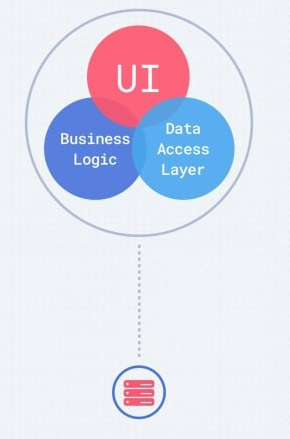
\includegraphics[scale=0.8]{mono}
	\caption{Exemplo da arquitetura monolítica \cite{imagensMonoMicro}.}
	\label{fig:exemplo1}
\end{figure}

\subsection{Arquitetura orientada a serviços}

A arquitetura orientada a serviços é uma evolução da arquitetura monolítica, por dividir a aplicação em serviços reutilizáveis que podem ser excetuados e implementados independentemente uns dos outros. Sendo que, estes podem estar conectados entre si, recorrendo a protocolos de comunicação. A escalabilidade é facilitada pela arquitetura, ao possibilitar o baixo acoplamento entre os componentes, facilitando a manutenção, reduz os custos e a complexidade \cite{serviços}.

\subsection{Arquitetura de microsserviços}

No caso, da arquitetura de microsserviços, este divide o sistema em pequenas aplicações, independentes umas das outras, ou seja, cada uma pode ser implementada e gerida individualmente, a essas aplicações dá-se o nome de microsserviços. Hoje em dia, esta arquitetura é muito utilizada devido ao crescente número de utilizadores, aumento de tráfego necessário e diferentes localizações desses mesmos utilizadores \cite{whymicroservices}.

As mais importantes caraterísticas de uma arquitetura de microsserviços são: a escalabilidade e a elasticidade. Sendo que, escalabilidade refere-se à capacidade de um sistema conseguir ajustar se ao crescimento no número de utilizadores ou no volume de dados sem comprometer o desempenho, ou a disponibilidade. A escalabilidade pode ser alcançada sem interromper o normal funcionamento do serviço mediante processos de escalabilidade horizontal, adicionar mais nós, ou vertical, aumentar a capacidade de processamento ou armazenamento de um, ou mais nós. Por outro lado, a elasticidade refere-se à capacidade de um sistema conseguir ajustar-se com as variações no tráfego ou carga de forma automática, aumentando ou diminuindo a alocação de recursos para algum serviço conforme os requisitos no momento. Normalmente esta gestão de alocar automaticamente recursos é feita por meio de contentores \cite{escalabilidade} \cite{escalabilidade1}.

Normalmente esta arquitetura está associada a padrões de \textit{software} como, por exemplo \ac{cqrs} (Segregação de Responsabilidade de Comando e Consulta), onde as responsabilidades da aplicação são divididos em dois blocos, o bloco das operações que modificam dados e o bloco que apresenta os dados da aplicação \cite{cqrs} e \textit{Database Per Service} (base de dados por serviço), em que cada aplicação contém uma base de dados, com os dados estritamente necessários para o seu correto funcionamento e funciona como um tipo de \textit{backup}, dado a redundância de dados \cite{database}.

A arquitetura de microsserviços apresenta flexibilidade em relação a modificações, dado o seu baixo acoplamento entre módulos e previne o colapso total do sistema no caso de erro ou falha. No entanto, isso exige um trabalho extra na implementação da comunicação entre serviços, o que pode causar uma complexidade na implementação e construção dos serviços, como também na própria implementação dos serviços devido a sua quantidade \cite{monoliticoVandDes}.

A figura \ref{fig:exemplo2} é um exemplo de uma aplicação construida com a arquitetura de microsserviços, apresenta-se dividido em vários microsserviços e em várias bases de dados.

\begin{figure}[H]
	\centering
	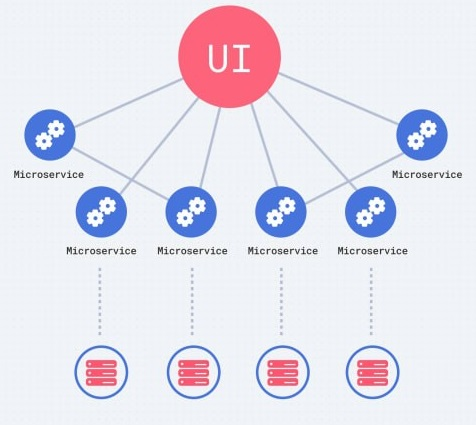
\includegraphics[scale=0.8]{micro}
	\caption{Exemplo da arquitetura de microsserviços \cite{imagensMonoMicro}.}
	\label{fig:exemplo2}
\end{figure}

\subsection{Arquitetura orientada a eventos}

Numa arquitetura orientada a eventos, os diferentes componentes do sistema, comunicam entre si recorrendo a eventos, eventos esses que podem ser alterações ou criação de elementos da lógica de negócio. Esta arquitetura recorre ao modelo de publicação e subscrição, onde os eventos são enviados através dos publicadores e recebidos pelos subscritores que subscreveram esse mesmo tipo de evento \cite{eventos}.

A figura \ref{fig:exemplo3} é um exemplo de como se processa eventos numa aplicação com uma arquitetura orientada a eventos.

\begin{figure}[H]
	\centering
	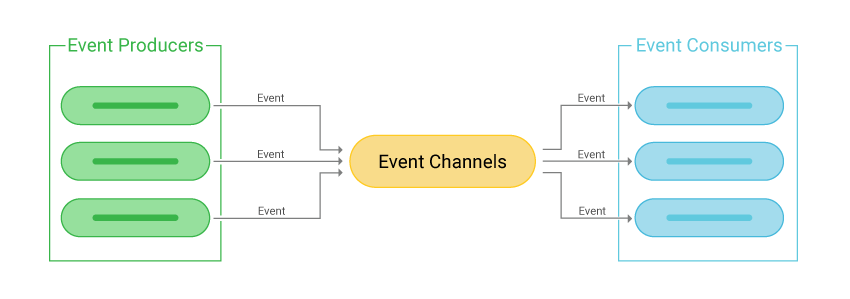
\includegraphics[scale=0.5]{event}
	\caption{Exemplo da arquitetura orientada a eventos \cite{event}.}
	\label{fig:exemplo3}
\end{figure}

\section{Comunicação entre serviços}

Numa arquitetura, com várias aplicações, muita vezes é preciso fazer passar dados entre elas ou mesmo verificar a existência das mesma e por isso tem se que recorrer os vários tipos de comunicações, como, por exemplo, comunicação síncrona e comunicação assíncrona. 

\subsection{Comunicação síncrona}

A comunicação síncrona é denominada comunicação bloqueante, dado que esta, está sempre a esperar uma resposta por parte do recetor do pedido, independentemente do tipo de dados, seja ele uma mensagem de erro como uma mensagem a confirmar a criação de algum tipo de dado e os respetivos atributos.

Começando com o \ac{rpc}, dado que é o mais antigo deles todos, neste caso a comunicação é feita mediante procedimento remoto entre servidor e cliente. Visto que o \textit{RPC} é uma comunicação de alto nível, esta facilita a implementação da mesma, pois a comunicação ao nível do protocolo \ac{tcp} é escondida, fazendo com que a desempenho seja maior. Sendo que é feita uma chamada de procedimento remoto, é necessário voltar a desenvolver ou escrever código, mas o esforço necessário é mínimo, devido que se pode reutilizar funcionalidades \cite{rpc}.

Passando ao \ac{soap}, este já é um protocolo especifico para comunicação de dados estruturados, com a limitação de só poder receber dados do tipo \ac{xml}. Comparando com \textit{RPC}, este apresenta uma complexidade maior na sua arquitetura \cite{SOAPREST}.

No que diz respeito ao \ac{grpc}, este é uma evolução do \textit{RPC}, de outro modo, uma \textit{framework}(ferramenta que auxilia no desenvolvimento de aplicação visto já conter código já definido) do \textit{RPC} tendo sido desenvolvido para combater alguns dos problemas do seu antecessor. A empresa \textit{GOOGLE}, a empresa que a desenvolveu, decidiu implementar, \textit{Protocol Buffers}(descreve a estrutura dos dados) para serializar informação e fazendo assim que microsserviços consigam comunicar entre si com auxílio desta ferramenta \cite{gRPC}.

Por meio de \ac{rest}, o servidor disponibiliza ao cliente uma interface de operações bem definidas, com ajuda do protocolo HTTP. Normalmente são usadas operações \ac{crud}, ou seja, operações de criação, leitura, atualização e destruição. Uma das vantagens é que o servidor permite que o cliente acesse as funcionalidades sem que este tenha conhecimento da implementação da mesma \cite{SOAPREST}.


\subsection{Comunicação assíncrona}

A comunicação assíncrona é denominada de uma comunicação não bloqueante, sendo que a aplicação não fica a espera de uma resposta imediata e prossegue com o normal funcionamento do programa.
Exemplos desse tipo de comunicação são: 
\begin{itemize}
    \item \ac{rabbitmq}
    \item \textit{Apache Kafka}
\end{itemize}

Sendo o \textit{RabbitMQ} um método de comunicação assíncrona, a sua utilização é normalmente associada a uma arquitetura orientada a eventos, sendo que, a esta pode também estar associada a uma arquitetura de microsserviços. Neste método a mensagem pode ser propagada ou enviada para um consumidor em específico. No caso de ser enviada para vários remetentes, a mensagem parte de um produtor, no qual, envia para uma \textit{exchange}, que por sua vez vai contar o número de serviços que subscreveram aquele tipo de mensagem, cria \textit{queues} respondente ao número contado com a informação enviada pelo produtor, os consumidores detetam uma nova entrada na \textit{queue}, consumem-na e tratam-na a seguir. Por outro lado, se a mensagem for enviada em que só haverá um remetente, o processo é semelhante, a mensagem parte do consumidor é enviado para a \textit{exchange}, a \textit{exchange} cria só uma \textit{queue} com a informação, o consumidor deteta a nova entrada na \textit{queue}, consume a e trata a seguir \cite{rabbit}.

O \textit{Apache Kafka} tem um funcionamento parecido ao \textit{RabbitMQ} apesar que as mensagens em vez de serem armazenadas em \textit{queues} são armazenadas em \textit{logs}. No caso das queues, as mensagens são eliminadas após a entrega das mesma aos consumidores e receberem um \textit{acknowledgment} por parte do mesmo, de outra forma, as \textit{logs} são mantidas num ficheiro e com ajuda de um apontador, o consumidor sabe qual foi a última mensagem consumida, evitando assim a duplicação da mesmas mensagens \cite{kafka}.

Comparando as duas opções, o \textit{Apache Kafka} devido as suas capacidades é mais adequado para casos em que há uma abundante de dados a serem transferidos enquanto, por outro lado, o \textit{RabbitMQ} é usado em casos que se espera que as transferências de mensagens sejam feitas com uma latência baixa.


\section{Tecnologias}

Nesta secção será feita uma introdução às tecnologias envolventes no projeto desenvolvido, explicando as suas funcionalidades, importância e alternativas disponíveis, tendo sempre em consideração alternativas \textit{open source}. 

Esta secção está dividida nas seguintes subsecções:

\begin{enumerate}
    \item Gestor de \textit{containers}
    \item Formato de troca de dados
    \item Autenticação
    \item Base de dados
    \item Cliente \textit{web}
    \item Ferramenta de teste de desempenho
\end{enumerate}

\subsection{Gestor de \textit{containers}}
No que diz respeito aos gestores de \textit{containers}, estes são pedaços de \textit{software} que ajudam na construção, desenvolvimento e gestão de \textit{containers}.

Cada \textit{container} é um espaço isolado, no qual, está incluído o código e dependências necessárias para o seu funcionamento. Os \textit{containers} são leves, portáveis e dado as suas caraterísticas funciona independentemente do ambiente no qual está inserido.

Exemplos de alguns dos gestores de \textit{containers} mais utilizados são:
\begin{itemize}
    \item \textit{Podman} \cite{podman}
    \item \textit{Docker} \cite{docker}
\end{itemize}


O \textit{Podman} e o \textit{Docker} são duas ferramentas usadas para gestão de \textit{containers} em \textit{DevOps}. Embora tenham funções semelhantes, existem diferenças importantes entre eles \cite{podmanVsDocker}.

Em termos de arquitetura, o \textit{Podman} não requer um \textit{daemon} (software que executa como um processo em plano de fundo \cite{daemon}) para chamar e gerir \textit{containers}, enquanto o Docker depende do \textit{daemon} para lidar com imagens, \textit{containers}, redes e armazenamento. O \textit{Podman} usa Pods para gerir \textit{containers} e permite a execução dos mesmos sem a necessidade de permissões de \textit{root} \cite{podmanVsDocker}.

O Docker requer permissões de \textit{root} para gerir \textit{containers}, por depender do \textit{daemon}. No entanto, numa atualização recente, o Docker introduziu a execução sem permissões de \textit{root}. No entanto, ainda são necessárias algumas configurações e pacotes de terceiros para executar \textit{containers} sem permissões de \textit{root} no Docker \cite{podmanVsDocker}.

Relativamente à segurança, o Docker apresenta riscos de segurança, pois, se alguém ganhar acesso a um \textit{container}, poderá comprometer os vários componentes com o mesmo acesso de \textit{root}. O \textit{Podman} é considerado mais seguro nesse aspeto, pois um invasor só poderá prejudicar os \textit{containers} aos quais tem acesso, sem ganhar acesso de \textit{root} \cite{podmanVsDocker}.

O \textit{Docker} não é apenas capaz de gerir \textit{containers}, mas também de criar imagens. Já o \textit{Podman} é projetado apenas para executar e gerir \textit{containers} \cite{podmanVsDocker}.

Em termos de suporte externo, o \textit{Docker} suporta o \textit{Docker Swarm} para orquestrar de \textit{containers}, permitindo executar um cluster de nós \textit{Docker} e implantar aplicações escaláveis sem dependências externas. O \textit{Podman} não suporta o \textit{Docker Swarm}, mas pode ser combinado com o \textit{Nomad}, que inclui um \textit{driver} para o \textit{Podman}. Além disso, o \textit{Docker} suporta o \textit{Docker Compose} para gerir aplicativos com vários \textit{containers} num único \textit{host}, enquanto o \textit{Podman} possui o \textit{Podman Compose} como alternativa \cite{podmanVsDocker}.

A abordagem de trabalho também difere entre o \textit{Podman} e o \textit{Docker}. O \textit{Docker} é independente e pode executar todas as tarefas necessárias de forma autónoma, enquanto o \textit{Podman} adota uma abordagem modular e recorre a várias integrações para realizar diferentes funções \cite{podmanVsDocker}.

\subsection{Formato de troca de dados}

Relativamente a formatos de troca de dados em aplicações \textit{web}, estes são independentes da plataforma, com uma importância elevada, dado que, conseguem ser lidos e usados por outras aplicações, ou mesmo tempo que, permitem que essa comunicação entre aplicações ou sistemas sejam feitas de forma segura e confiável. Além disso, o uso destes tipos de formatos de trocas de dados proporcionam uma certa flexibilidade.

Alguns exemplos de formatos de troca de dados são: XML, \ac{json}, \ac{yaml} e \ac{csv}. 

O formato de trocas de dados XML foi uma das primeiras formatos a surgirem, precisamente em 1998. Apesar de novas linguagens de configuração estarem a ultrapassar o XML ainda existem muitas situações em que a natureza estruturada do XML e a sua flexibilidade funcionam melhor para configurações complexas \cite{formatosDeDados}.

Na Listagem \ref{lst:xml} é apresenta um exemplo de forma XML.

\begin{minipage}{0.9\linewidth}
\begin{lstlisting}[language=xml, caption=Exemplo do formato XML. , label=lst:xml]
<people>
  <person>
    <id>1</id>
    <nome>Exemplo1</nome>
    <idade>25</idade>
  </person>
  <person>
    <id>2</id>
    <nome>Exemplo2</nome>
    <idade>30</idade>
  </person>
  <person>
    <id>3</id>
    <nome>Exemplo3</nome>
    <idade>40</idade>
  </person>
</people>
\end{lstlisting}
\end{minipage}

Em relação a desvantagens e vantagens, as vantagens do XML, são:
\begin{itemize}
    \item Existem esquemas para a validação e criação de tipos personalizados
    \item Permite facilmente a realização de diferentes formatos a partir de uma sintaxe comum \cite{formatosDeDados}
\end{itemize}

Por sua vez as desvantagens do XML são:
\begin{itemize}
    \item Não é considerado facilmente legível por humanos devido à natureza descritiva dos elementos.
    \item Detalhada (aumenta a capacidade de armazenamento e as necessidades de largura de banda) e contém frequentemente sintaxe redundante \cite{formatosDeDados}
\end{itemize}

No caso do JSON, este existe desde do início dos anos 2000 e reconhecido como uma especificação formal em 2013. É derivado da linguagem de programação JavaScript, mas independente dessa linguagem. Apresenta-se como uma alternativa mais simples em relação a muitos outros formatos e como uma das linguagens mais utilizados no momento \cite{formatosDeDados}. 

Na Listagem \ref{lst:json} é apresenta um exemplo de forma JSON.

\begin{minipage}{0.9\linewidth}
\begin{lstlisting}[language=json, caption=Exemplo do formato JSON., label=lst:json]
[
  {
    "id": 1,
    "nome": "Exemplo1",
    "idade": 25
  },
  {
    "id": 2,
    "nome": "Exemplo2",
    "idade": 30
  },
  {
    "id": 3,
    "nome": "Exemplo3",
    "idade": 40
  }
]
\end{lstlisting}
\end{minipage}

Em relação a desvantagens e vantagens, as vantagens do JSON, são:
\begin{itemize}
    \item Facilmente legível por humanos
    \item Sintaxe simples 
    \item Rápido para ser analisado dado a sua marcação limitada \cite{formatosDeDados}
\end{itemize}

Por sua vez as desvantagens do JSON são:
\begin{itemize}
    \item Suporte limitado em relação a tipo de dados
    \item Não suporta configurações complexas
    \item Não suporta comentários de suporte aos atributos \cite{formatosDeDados}
\end{itemize}

Por outro lado, o YAML foi criado em 2001. Embora o YAML tenha um aspeto diferente do JSON, o YAML é um superconjunto do JSON. Como um superconjunto de JSON, um ficheiro YAML válido pode conter JSON. Além disso, o JSON também pode transformar-se em YAML. O próprio YAML também pode conter JSON nos seus ficheiros de configuração \cite{formatosDeDados}.

Na Listagem \ref{lst:yaml} é apresenta um exemplo de forma YAML.

\begin{minipage}{0.9\linewidth}
\begin{lstlisting}[language=yaml, caption=Exemplo do formato YAML. , label=lst:yaml]
- id: 1
  nome: Exemplo1
  idade: 25
- id: 2
  nome: Exemplo2
  idade: 30
- id: 3
  nome: Exemplo3
  idade: 40
\end{lstlisting}
\end{minipage}


Em relação a desvantagens e vantagens, as vantagens do YAML, são:
\begin{itemize}
    \item Sintaxe Legível por humanos
    \item Sintaxe compacta
    \item Suporta tipos de objetos independentes de idioma \cite{formatosDeDados}
\end{itemize}

Por sua vez as desvantagens do YAML são:
\begin{itemize}
    \item O formato de indentação é propenso a erros de sintaxe e validação
    \item A portabilidade com certos tipos pode não existir devido à falta de recursos em todos os idiomas
    \item A depuração é difícil
    \item Pontos de interrupção e funcionalidade semelhante não existem \cite{formatosDeDados}
\end{itemize}

Por último, o CSV. Os arquivos CSV são arquivos de texto que utilizam vírgulas para separar os valores, e são amplamente utilizados em softwares de escritório como o Microsoft Excel \cite{csvConteudo}. Eles normalmente contêm uma linha de cabeçalho que fornece nomes de coluna para os dados, mas de outra forma, são considerados semiestruturado \cite{csvDesvantagenseInfo}.

Na Listagem \ref{lst:csv} é apresenta um exemplo de forma CSV.

\begin{minipage}{0.9\linewidth}
\begin{lstlisting}[language=csv, caption=Exemplo do formato CSV., label=lst:csv]
id,nome,idade
1,Exemplo1,25
2,Exemplo2,30
3,Exemplo3,40
\end{lstlisting}
\end{minipage}

Em relação a desvantagens e vantagens, as vantagens do CSV, são:
\begin{itemize}
    \item O formato CSV é simples e de fácil compreensão
    \item O CSV é amplamente suportado por diferentes softwares e sistemas operativos
    \item Os arquivos CSV tendem a ter um tamanho menor em comparação com outros formatos Os arquivos CSV são formatados como texto legível \cite{csvVantagens}
\end{itemize}

Por sua vez as desvantagens do CSV são:
\begin{itemize}
    \item Nenhuma restrição no modelo de dados, pode resultar em dados corrompidos
    \item Não se adapta bem ao trabalhar com \textit{Big Data}. Geralmente, eles não podem ser divididos em partições para processamento paralelo e não podem ser compactados tão bem quanto formatos binários
    \item Talvez seja necessário aplicar um esquema nos dados semiestruturados para facilitar a consulta e análise \cite{csvDesvantagenseInfo}
\end{itemize}

\subsection{Autenticação}
A decisão de fazer a implementação de um sistema de autenticação é crucial para a segurança do sistema inteiro, seja em aplicações públicas como em aplicações privadas. Estes sistemas de autenticação tem o propósito de assegurar a manipulação de dados não desejados e a visualização dos mesmos se assim for o objetivo da mesma aplicação. 

Para isso existem alguns formatos de autenticação que ajudam nessa tarefa de realizar a autenticação, como, por exemplo:
\begin{itemize}
    \item \ac{jwt}
    \item Chaves \ac{api}
\end{itemize}

Começando com o JWT, este é um padrão que define a transferência de dados entre duas partes recorrendo a uma token passado mediante um \textit{HTTP Header}. Este mesmo token é gerado por meio de uma chave privada e acessados com uma chave publica sendo composto por três componentes: \textit{Header}, \textit{Payload} e \textit{Signature}. O \textit{Header} contém informações sobre o algoritmo usado para criar o \textit{hash} e o tipo de \textit{token}, o \textit{Payload} contém \textit{claims} como, por exemplo, objetos \textit{JSON}, data de expiração, quem emitiu o \textit{token} e outras informações adicionais, e a \textit{Signature} é a junção dos \textit{hashes} gerados \cite{jwt}.

E finalmente, as chaves API estas são códigos únicos fornecidos ao utilizador que identificam o mesmo. As chaves API são um bom meio de controlo e supervisão do sistema, visto que, pode prevenir o abuso da API por meio de restrições e utilizadores maliciosos. Comparando com o exemplo apresentado anteriormente, este tipo de autenticação é menos segura \cite{apikeys}.

\subsection{Base de dados}
No que diz respeito, a base de dados é uma ferramenta necessária para o armazenamento e consulta desses mesmo dados. Atualmente são utilizadas dois tipos de bases de dados, bases de dados relacionais e as bases de dados não relacionais.

Em relação a bases de dados relacionais, como o nome indica, os dados são armazenados recorrendo a relações entre tabelas, enquanto bases de dados não relacionais armazenam os dados de forma não estruturada.

Fazendo uma análise mais profunda, uma base de dados relacional é uma boa escolha para aplicações que envolvem a manipulação de várias transações. Apesar de não ter sido desenvolvida com a arquitetura \ac{oop} em mente, é preciso fazer uma configuração das chaves primárias e estrangeiras para contornar o problema. 

Em contrapartida, uma base de dados não relacional é usada em situações que as aplicações geram um grande tráfego de dados, devido à sua alta escalabilidade e a ter um desempenho superior em comparação ao as bases de dados relacionais.

Alguns exemplos de base de dados são:
\begin{itemize}
    \item \ac{mysql} (Base de dados relacional) \cite{mysql}
    \item \ac{mariadb} (Base de dados não relacional) \cite{mariadb}
\end{itemize}

\subsection{Cliente \textit{web}}
Relativamente a clientes \textit{web} estes são ferramentas importantes de interação com servidores \textit{web}. Por pedidos http ou https (métodos do tipo \textit{GET}, \textit{POST}, \textit{PUT}, \textit{DELETE}, etc) é possível obter a resposta ao pedido feito, guardá-la e até comparar a resposta com testes desenvolvidos para assegurar o funcionamento normal da aplicação e que as regras de negócio foram implementadas. Além disso, também é possível averiguar se houve regressão na qualidade do código por meio de testes de regressão, dado que a adição de uma nova funcionalidade pode causar problemas numa funcionalidade já existente.

Alguns exemplos de clientes \textit{web} são:
\begin{itemize}
    \item \textit{Postman} \cite{postaman}
    \item \textit{Insomnia (Open source)} \cite{insomnia}
\end{itemize}

Comparando as duas aplicações, \textit{Postman} aparenta ter um conjunto de funcionalidades mais maduras relativamente à aplicação \textit{Insomnia}.


A seguir será enumerado as funcionalidades que fazem o \textit{Postman} se destingir das outras ferramentas de teste: 

\begin{itemize}
    \item Documentação de API: Consegue gerar facilmente documentação da \textit{API} \cite{postmanvsInsomnia}
    \item Execuções de coleções: Recorrendo a coleções é possível executar um grupo de pedidos como uma série, sendo esta funcionalidade bastante necessária para os testes automáticos \cite{postmanvsInsomnia}
    \item Monitorização: Periodicamente é possível executar uma coleção e verificar as suas respostas e desempenho \cite{postmanvsInsomnia}
    \item Testes em JavaScript: Permite desenvolver testes recorrendo a \textit{JavaScript} \cite{postmanvsInsomnia}
    \item Servidores fictícios: Fornece servidores fictícios que permitem a simulação de cada um dos \textit{endpoints}, sem que seja preciso desenvolver o próprio serviço \cite{postmanvsInsomnia}
\end{itemize}

Por outro lado, será enumerado as funcionalidades únicas ao \textit{Insomnia}:

\begin{itemize}
    \item Suporte a \textit{plugins}: Permite o uso e a criação de novos \textit{plugins} \cite{postmanvsInsomnia}
    \item Certificados de cliente e validação SSL: suporta a atribuição de certificados de cliente a espaços de trabalho e fornece opções de validação SSL \cite{postmanvsInsomnia}
    \item Geração de pedaços de código: Consegue gerar pedaços de código em 12 linguagens de programação diferentes \cite{postmanvsInsomnia}
    \item Visualização avançada de respostas: Permite aos utilizadores visualizar respostas para além dos formatos \textit{JSON} e \textit{XML}. Suporta vários tipos de conteúdo, como páginas \textit{HTML}, imagens, \textit{SVGs}, ficheiros de áudio e até documentos \textit{PDF} \cite{postmanvsInsomnia}
\end{itemize}


\subsection{Ferramenta de teste de desempenho}

Apesar de ser importante testar a aplicação relativamente às regras de negócio, da mesma forma é importante testar a desempenho da mesma, utilizando aplicações de teste de desempenho que simulam a quantidade de utilizadores definida pelos requisitos não funcionais a usar uma certa funcionalidade ou várias funcionalidades de uma certa aplicação, ou aplicações em simultâneo. A mesma consegue apresentar relatórios, incluindo na mesma, gráficos dos pedidos feitos ao longo do tempo em que o, tempos máximos, mínimos e médios.

Exemplo de aplicações de teste de desempenho:
\begin{itemize}
    \item JMeter \cite{jmeter}
    \item \ac{soapui} \cite{soapui}
\end{itemize}

O \textit{SoapUI} e o \textit{JMeter} têm objetivos e pontos fortes diferentes. No caso, do \textit{SoapUI}, este é utilizado principalmente para testes funcionais de serviços Web e APIs, enquanto o \textit{JMeter} é especializado em testes de desempenho, nomeadamente testes de carga. Por outro lado, o \textit{SoapUI} oferece uma interface amigável com fácil importação e o \textit{JMeter} tem uma interface de utilizador baseada em formulários com características especificamente concebidas para APIs e aplicações Web. Em relação a relatórios, o \textit{SoapUI} gera relatórios automaticamente e a sua versão paga oferece informações mais detalhadas e o \textit{JMeter} não possui funcionalidades de relatório incorporadas, exigindo que os utilizadores realizem os relatórios manualmente \cite{soapuivsJmeter}.

Tanto o \textit{SoapUI} como o \textit{JMeter} têm limitações. No \textit{SoapUI}, os testes de carga exigem um esforço significativo de programação para criar testes e simulações de cenários. O \textit{SoapUI} também consome uma grande quantidade de memória ao gerar uma carga pesada, levando a problemas de desempenho. O \textit{JMeter} não possui recursos de relatório integrados, essenciais para identificar gargalos de desempenho e otimizar o desempenho. A sua interface de utilizador também é considerada menos fácil de utilizar e pode ser difícil de trabalhar \cite{soapuivsJmeter}.

\section{Padrões}
\subsection{\textit{Database Per Service}}

Imaginemos que está a ser desenvolvida uma loja de comércio online em que é recorrido à arquitetura de microsserviços. Cada serviço precisa de persistir as informações. Como, por exemplo, o serviço que disponibiliza funcionalidades para a gestão de encomendas grava informações acerca das encomendas enquanto outro serviço como, por exemplo, o serviço que disponibiliza funcionalidades para a gestão de produtos grava informações acerca dos produtos \cite{databasePerServicePattern}.

O problema que surge neste caso é o seguinte: Qual será a arquitetura da base de dados numa aplicação de microsserviços? \cite{databasePerServicePattern}.

Tendo em conta que:

\begin{itemize}
    \item Os serviços devem ser desacoplados entre si, ou seja, ser desenvolvidos, implementados e dimensionados de forma independente \cite{databasePerServicePattern}
    \item Pode ser necessário efetuar consulta de dados a outros serviços \cite{databasePerServicePattern}
    \item Pode ser necessário unir dados pertencentes a outros serviços \cite{databasePerServicePattern}
    \item As bases de dados podem ser replicadas \cite{databasePerServicePattern}
    \item Cada serviço pode ter requisitos diferentes dos outros serviços \cite{databasePerServicePattern}
\end{itemize}

A solução para o problema descrito em cima passa por cada serviço ter a responsabilidade de persistência dos próprios dados. Estes mesmos, passam a estarem privados e só podem ser acedidos através do serviço que os mantém, ou seja, os dados não podem ser acessados diretamente pelos os outros serviços \cite{databasePerServicePattern}.

Existem três opções para manter esses dados privados como, por exemplo:

\begin{itemize}
    \item Tabelas privadas por serviço: Cada serviço possui um conjunto de tabelas que devem ser acessadas apenas por esse serviço \cite{databasePerServicePattern}
    \item Esquema por serviço: Cada serviço possui um esquema de banco de dados privado para esse serviço \cite{databasePerServicePattern}
    \item Servidor de base de dados por serviço: Cada serviço possui um servidor de banco de dados \cite{databasePerServicePattern}
\end{itemize}

Para uma menor sobrecarga as melhores opções são as tabelas privadas por serviço e esquema por serviço, por outro lado, se houver a necessidade em que alguns serviços precisem de alto desempenho a melhor é o servidor de base de dados por serviço \cite{databasePerServicePattern}.

O uso de uma base de dados por serviço tem as seguintes vantagens:
\begin{itemize}
    \item Os serviços tornam-se desacolados \cite{databasePerServicePattern}
    \item Alterações na base de dados de um serviço não afetam os outros serviços \cite{databasePerServicePattern}
    \item Cada serviço pode usar a base de dados mais adequada às necessidades do serviço \cite{databasePerServicePattern}
\end{itemize}

Por sua vez tem as seguintes desvantagens:
\begin{itemize}
    \item Dificuldade na junção de dados de várias bases de dados \cite{databasePerServicePattern}
    \item Complexidade na gestão de várias bases de dados \cite{databasePerServicePattern}
\end{itemize}

E finalmente, relativamente a padrões relacionados temos os seguintes:
\begin{itemize}
    \item \textit{API Composition}: Permite a junção de dados 
    \item \textit{CQRS}: Divide responsabilidades em serviços de consulta e serviços de escrita 
    \item \textit{Saga}: Implementa as transações entre serviços  
    \item Arquitetura de microsserviços: Cria a necessidade para o uso deste padrão 
\end{itemize}

\subsection{\textit{Saga}}
Imaginemos que foi aplicado o padrão descrito anteriormente, ou seja, cada serviço tem a sua própria base de dados. Sendo que algumas transações são espalhadas pelos vários serviços é preciso um mecanismo para fazer a implementação dessas mesmas. Como, por exemplo, usando o paradigma anterior, o cliente tem alguma restrição na conta, quando este fizer algum pedido a aplicação deve garantir que a encomenda tenha em conta a restrição do cliente \cite{sagaPattern}.

O problema que surge neste caso é o seguinte: Como será implementada as transações? \cite{sagaPattern}

A solução para o problema descrito em cima passa por implementar cada transação que abrange vários serviços como um \textit{SAGA}, sequencia de transações locais. Cada transação local atualiza o banco de dados do serviço onde se encontra e publica o evento para acionar a próxima transação. No caso de alguma transação local violar as regras de negócio será executado transações que vão reverter as alterações feitas realizadas pelas transações anteriores \cite{sagaPattern}.

O uso deste padrão tem as seguintes vantagens:
\begin{itemize}
    \item Possível manter a consistência de dados entre serviços \cite{sagaPattern}
\end{itemize}

Por sua vez tem as seguintes desvantagens:
\begin{itemize}
    \item Sistema mais complexo \cite{sagaPattern}
\end{itemize}

E finalmente, relativamente a padrões relacionados temos os seguintes:
\begin{itemize}
    \item \textit{Database Per Service}
    \item \textit{Event sourcing}
    \item \textit{Domain event}
\end{itemize}

\subsection{\textit{CQRS}}

Imaginemos que foi implementado a arquitetura de microsserviços e \textit{Database Per Service}, como resultado pode resultar em problemas de divergência, escabilidade e desempenho \cite{cqrsPattern}.

O problema que surge neste caso é o seguinte: Como será feita a implementação dos serviços? \cite{cqrsPattern}

A solução para o problema descrito em cima passa por dividir um serviço, com todas as funcionalidades (\textit{POST/GET/PUT/DELETE}) em dois serviços em que um dele terá a responsabilidade de fazer leituras e o outro por fazer escritas \cite{cqrsPattern}.

O uso deste padrão tem as seguintes vantagens:
\begin{itemize}
    \item Separação de responsabilidades \cite{cqrsPattern}
    \item Promove a possível de escabilidade dos serviços \cite{cqrsPattern}
\end{itemize}

Por sua vez tem as seguintes desvantagens:
\begin{itemize}
    \item Aumenta a complexidade do projeto \cite{cqrsPattern}
    \item Duplicação de código \cite{cqrsPattern}
\end{itemize}

E finalmente, relativamente a padrões relacionados temos os seguintes:
\begin{itemize}
    \item \textit{Database Per Service} 
    \item \textit{API Composition} 
\end{itemize}

\subsection{\textit{API Composition}}

Imaginemos que foi implementado a arquitetura de microsserviços e \textit{Database Per Service}. Como resultado, a implementação de pesquisas para juntar dados de vários serviços torna-se mais difícil \cite{apiCompositionPattern}. 

O problema que surge neste caso é o seguinte: Como implementar essas pesquisas numa arquitetura de microsserviços? \cite{apiCompositionPattern}

A solução para o problema descrito em cima passa por implementar um \textit{Composer API}, que invocará os serviços necessários e realizará a junção desses mesmos dados \cite{apiCompositionPattern}.

O uso deste padrão tem as seguintes vantagens:
\begin{itemize}
    \item Torna-se mais simples consultar dados \cite{apiCompositionPattern}
\end{itemize}

Por sua vez tem as seguintes desvantagens:
\begin{itemize}
    \item Algumas consultas resultariam em junções ineficientes de grandes conjuntos de dados \cite{apiCompositionPattern}
\end{itemize}

E finalmente, relativamente a padrões relacionados temos os seguintes:
\begin{itemize}
    \item \textit{Database Per Service}
    \item \textit{CQRS}
\end{itemize}

\subsection{\textit{Messaging}}

Imaginemos que foi implementado a arquitetura de microsserviços e que os serviços precisam de um protocolo de comunicação entre processos \cite{messagingPattern}. 

O problema que surge neste caso é o seguinte: Como os serviços comunicam-se entre si? \cite{messagingPattern}

A solução para o problema descrito em cima passa por usar mensagens assíncronas para a comunicação entre serviços. Existem vários estilos de comunicação assíncrona, tais como:

\begin{itemize}
    \item \textit{Request/response}: Um serviço envia uma mensagem a outro serviço e espera receber uma resposta imediatamente \cite{messagingPattern}
    \item \textit{Notifications}: Um remetente envia uma mensagem a um destinatário, mas não espera uma resposta. Nem um é enviado \cite{messagingPattern}
    \item \textit{Request/asynchronous response}: Um serviço envia uma mensagem de solicitação a outro serviço e espera receber uma resposta eventualmente \cite{messagingPattern}
    \item \textit{Publish/subscribe}: Um serviço publica uma mensagem para zero ou mais destinatários (subscritores) \cite{messagingPattern}
    \item \textit{Publish/asynchronous response}: Um serviço publica um pedido a um ou mais destinatários, alguns dos quais enviam uma resposta \cite{messagingPattern}
\end{itemize}

O uso deste padrão tem as seguintes vantagens:
\begin{itemize}
    \item Desacopla o remetente da mensagem \cite{messagingPattern}
    \item Suporta variedade de padrões de comunicação \cite{messagingPattern}
    \item Aumenta a disponibilidade, dado que, o \textit{message broker} faz de \textit{buffer}\cite{messagingPattern}
\end{itemize}

Por sua vez tem as seguintes desvantagens:
\begin{itemize}
    \item Aumenta a complexidade do sistema \cite{messagingPattern}
\end{itemize}

E finalmente, relativamente a padrões relacionados temos os seguintes:
\begin{itemize}
    \item \textit{SAGA}
    \item \textit{CQRS}
\end{itemize}

\subsection{\textit{API Gateway}}

Imaginemos que foi implementado a arquitetura de microsserviços no mesmo contexto de uma loja online e está a ser implementado uma certa pagina, por exemplo, uma página de um certo produto \cite{apiGatewayPattern}. Para cada página dessas é preciso obter, por exemplo, as seguintes informações:

\begin{itemize}
    \item Informações do produto, como nome, descrição, preço e fabricante \cite{apiGatewayPattern}
    \item Número de compras já realizadas \cite{apiGatewayPattern}
    \item Quantidade disponível em armazém \cite{apiGatewayPattern}
    \item Comentários efetuados pelos clientes que compraram o produto \cite{apiGatewayPattern}
    \item Data disponível para entrega do produto \cite{apiGatewayPattern}
    \item Entre outras informações \cite{apiGatewayPattern}
\end{itemize}

Para obter as várias informações e como a loja utiliza o padrão em cima referido, as informações estão espalhadas pelos diversos serviços \cite{apiGatewayPattern}. Por isso seria necessário realizar pedidos aos seguintes serviços:

\begin{itemize}
    \item Serviço das informações do produto 
    \item Serviço de compras 
    \item Serviço de inventário  
    \item Serviço de comentários
    \item Serviço de encomendas 
\end{itemize}

O problema que surge neste caso é o seguinte: Como os clientes acedem a cada um dos serviços numa aplicação baseada em microsserviços? \cite{apiGatewayPattern}

Tendo em conta que:

\begin{itemize}
    \item As informações diferem de cliente para cliente, a versão \textit{desktop} é mais elaborada que a versão \textit{mobile} \cite{apiGatewayPattern}
    \item O desempenho da rede difere de cliente para cliente \cite{apiGatewayPattern}
    \item As instâncias e o seu número mudam dinamicamente  \cite{apiGatewayPattern}
    \item A divisão da aplicação  pelos serviços deve ser oculto para os clientes \cite{apiGatewayPattern}
    \item Os serviços podem recorrer a um conjunto de diferentes protocolos \cite{apiGatewayPattern}
\end{itemize}


A solução para o problema descrito em cima passa por implementar uma \textit{API Gateway}, ou seja, um único ponto de acesso para todos os clientes \cite{apiGatewayPattern}. Os pedidos recebidos serão encaminhados para o correspondente serviço. Conforme apresentado na figura \ref{fig:gateway1}.

\begin{figure}[H]
	\centering
	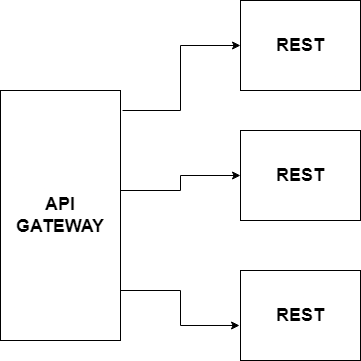
\includegraphics[scale=0.5]{gateway1.png}
	\caption{Exemplo de uma API Gateway.}
	\label{fig:gateway1}
\end{figure}

Por outro lado, uma variação à estrutura apresentada na figura anterior é a seguinte, cada tipo de cliente (Web, mobile e aplicação externa de terceiros) pode ter a sua própria \textit{API Gateway} \cite{apiGatewayPattern}. Conforme apresentado na figura \ref{fig:gateway2}.

\begin{figure}[H]
	\centering
	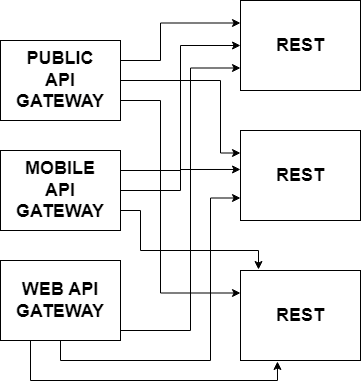
\includegraphics[scale=0.5]{gateway2.png}
	\caption{Exemplo de uma API Gateway.}
	\label{fig:gateway2}
\end{figure}

O uso deste padrão tem as seguintes vantagens:
\begin{itemize}
    \item Isola os clientes para a divisão dos microsserviços \cite{apiGatewayPattern}
    \item Adequa a necessidade de cada cliente \cite{apiGatewayPattern}
    \item Simplifica a chamada dos serviços \cite{apiGatewayPattern}
    \item Pode reduzir o número de pedidos \cite{apiGatewayPattern}
    \item O cliente não precisa de saber o endereço das instâncias dos serviços \cite{apiGatewayPattern}
\end{itemize}

Por sua vez tem as seguintes desvantagens:
\begin{itemize}
    \item Aumenta a complexidade do sistema \cite{apiGatewayPattern}
    \item O tempo de resposta aumenta devido aos saltos adicionais  \cite{apiGatewayPattern}
\end{itemize}

E finalmente, relativamente a padrões relacionados temos os seguintes:
\begin{itemize}
    \item \textit{Access token}
    \item \textit{API Composition}
\end{itemize}

\subsection{\textit{Access token}}

Imaginemos que foi implementado a arquitetura de microsserviços e o padrão \textit{API Gateway} \cite{accessTokenPattern}. 

O problema que surge neste caso é o seguinte: Como é comunicado a identidade do solicitador do pedido? \cite{accessTokenPattern}

A solução para o problema descrito em cima passa pela \textit{API Gateway} autenticar o pedido e passar o token de acesso (por exemplo, \textit{JWT}) que identifica a identidade do solicitador aos serviços \cite{accessTokenPattern}.

O uso deste padrão tem as seguintes vantagens:
\begin{itemize}
    \item Promove a segurança no sistema dado que assim a identidade do solicitador é conhecida \cite{accessTokenPattern}
    \item Os serviços aos saberem a identidade do solicitador podem dependendo das suas permissões, autorizar ou não autorizar a execução de uma operação/ação \cite{accessTokenPattern}
\end{itemize}

E finalmente, relativamente a padrões relacionados temos os seguintes:
\begin{itemize}
    \item \textit{API Gateway}
\end{itemize}